% !TEX program = pdflatex
% IEEE conference draft; no venue-specific page limit has been selected.
% The original manuscript is preserved as paper-crewai-original.tex.
% All numerical results refer to the partial study-20261009-v3.
\documentclass[conference]{IEEEtran}
\usepackage[T1]{fontenc}
\usepackage{cite}
\usepackage{amsmath,amssymb}
\usepackage{graphicx}
\usepackage{booktabs}
\usepackage{array}
\usepackage{url}
\usepackage{xcolor}
\usepackage{tikz}
\usetikzlibrary{arrows.meta,positioning,calc}
\graphicspath{{paper-figures/}}
\newcommand{\NEI}{\textsc{nei}}
\newcommand{\CI}{\textsc{ci}}
\newcommand{\modelname}{\texttt{gemma4:31b-cloud}}
\newcommand{\jevname}{\texttt{jev-1.13.0}}
\newcommand{\pct}{\%}

\begin{document}
\title{KajiAI: Auditable Claim Verification with Bounded Research and Selective Evidence Gates}

% Replace the fields below with the actual authors and affiliations.
\author{\IEEEauthorblockN{Author Name(s)}
\IEEEauthorblockA{\textit{Department and Institution}\\
City, Country\\
Email address or ORCID}}
\maketitle

\begin{abstract}
A correct factual prediction does not necessarily provide verifiable evidence, and additional web research can change a previously correct answer. This paper presents KajiAI, a LangGraph workflow that separates a language model's proposed verdict from an evidence-based acceptance decision. The workflow records versioned retrieved text, checks literal quotation provenance, applies structural evidence requirements and model-based citation review, and repeats research within explicit resource budgets. A quota-interrupted evaluation on the AVeriTeC development split produced 302 workflow attempts and 283 model-only attempts, including seven execution failures. On the 177 claims assessed in both conditions, the workflow achieved 63.3\pct\ label accuracy and 0.502 macro F1, compared with 49.2\pct\ and 0.413 for the model-only control. The paired accuracy difference was 14.1 percentage points, with a 95\pct\ bootstrap interval of 6.2--22.6 points. Across all workflow attempts, 19 verdicts passed the complete evidence gate; all matched the dataset labels, but coverage was only 6.3\pct. Additional rounds corrected eight predictions and changed 20 correct predictions into incorrect outcomes. These preliminary observations motivate evaluating prediction quality, acceptance coverage, evidence support and research cost separately. Contemporary web access, incomplete execution and the absence of independent human citation validation limit the conclusions.
\end{abstract}

\begin{IEEEkeywords}
automated fact-checking, retrieval-augmented generation, LangGraph, citation provenance, selective prediction, AVeriTeC
\end{IEEEkeywords}

\section{Introduction}
Automated fact-checking requires more than assigning a plausibly correct label. A system should identify evidence, connect that evidence to the claim, disclose uncertainty and preserve enough provenance for inspection. FEVER established an evidence-oriented task using claims derived from Wikipedia \cite{fever}. AVeriTeC extends this setting to real-world claims and web evidence \cite{averitec}. Its shared-task score combines verdict correctness with evidence quality \cite{sharedtask}, emphasizing that label agreement alone is an incomplete account of verification.

Retrieval-augmented generation provides external information to a language model \cite{rag}, but retrieved documents, citations and repeated reasoning do not themselves guarantee an evidence-supported verdict. Citation evaluation distinguishes answer correctness from citation quality \cite{alce}. This distinction motivates an architecture in which prediction and acceptance are observable, separate decisions.

We present KajiAI, an auditable workflow implemented with LangGraph. A model proposes a factual label and an evidence assessment. A gate checks retrieved citations, exact quotations, assertion coverage, source-host diversity and domain requirements, followed by automated semantic citation review. Failed checks preserve the prediction while withholding an accepted verdict. Unresolved gaps can trigger further research, subject to limits on rounds, searches, page fetches, elapsed time and reported tokens.

This paper examines three questions: \textbf{RQ1}, whether the complete workflow improves label prediction relative to the same model without retrieval; \textbf{RQ2}, how evidence checks affect coverage and accuracy among accepted verdicts; and \textbf{RQ3}, whether additional research improves saved predictions enough to justify its resource use.

The contributions are an explicit state-and-provenance design separating prediction from acceptance; a frozen, resumable evaluation protocol with failure-inclusive scoring and fixed-evidence policy replay; and preliminary measurements exposing the interaction between accuracy, selective acceptance and iteration cost. LangGraph is the orchestration mechanism, rather than a proposed new learning algorithm. The experiment does not isolate a framework migration or establish superiority over other fact-checking systems.

\section{Related Work}
\subsection{Evidence-Based Fact-Checking}
FEVER pairs supported and refuted claims with annotated evidence sentences \cite{fever}. AVeriTeC uses real-world claims, question--answer evidence and textual justifications from web sources \cite{averitec}. The AVeriTeC shared task evaluates evidence retrieval and veracity prediction jointly \cite{sharedtask}. We use its development labels for a local four-class study; our scores are not official AVeriTeC scores and cannot be directly compared with shared-task rankings.

\subsection{Retrieval and Citation Evaluation}
Lewis et al.\ introduced a retrieval-augmented formulation combining parametric generation with an external document memory \cite{rag}. Self-RAG learns retrieval and critique behaviors using reflection tokens \cite{selfrag}. KajiAI does not train such a model: its research loop uses structured assessments, query templates and explicit routing rules. This makes the behavior inspectable while leaving query generation and stopping quality open to evaluation.

ALCE evaluates generated answers along fluency, correctness and citation quality dimensions \cite{alce}. Our literal-quote check addresses a narrower property: whether a quoted string occurs in stored text for its cited URL. A separate model reviews whether that quotation supports its attached finding. Neither mechanism independently establishes the truth of the overall verdict.

\subsection{Selective Prediction}
Selective classification introduces a reject option to trade coverage for accuracy on accepted instances \cite{selective}. KajiAI applies this perspective through evidence requirements rather than a learned selective classifier. We report coverage and conditional label accuracy without importing statistical risk guarantees from selective-learning methods. Model confidence categories and citation-review confidence have not been calibrated against independent human judgments.

\section{System Design}
\subsection{Stateful Graph and Execution}
LangGraph supports stateful workflows combining deterministic operations and model calls \cite{langgraph}. Eight nodes execute KajiAI's process in Fig.~\ref{fig:architecture}. The shared state includes the original claim, optional reference date, domain, assertions, retrieval ledger, research history, proposed assessment, evidence gaps, budgets and stop reason. Individual claims follow a sequential graph; the study runner processes up to three claims concurrently.

\begin{figure}[t]
\centering
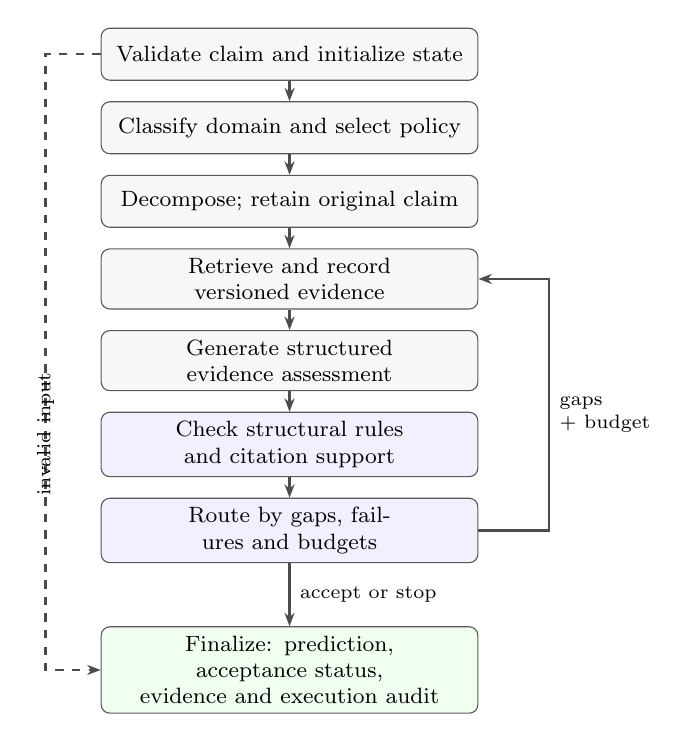
\begin{tikzpicture}[
  node distance=2.6mm,
  flowblock/.style={draw=black!65, rounded corners=1.1mm,
    fill=black!3, align=center, text width=4.55cm,
    minimum height=6.6mm, font=\footnotesize},
  flowgate/.style={flowblock, fill=blue!6},
  flowarrow/.style={-{Stealth[length=1.7mm]}, thick, draw=black!70}
]
\node[flowblock] (validate) {Validate claim and initialize state};
\node[flowblock, below=of validate] (classify) {Classify domain and select policy};
\node[flowblock, below=of classify] (decompose) {Decompose; retain original claim};
\node[flowblock, below=of decompose] (retrieve) {Retrieve and record versioned evidence};
\node[flowblock, below=of retrieve] (analyze) {Generate structured evidence assessment};
\node[flowgate, below=of analyze] (check) {Check structural rules and citation support};
\node[flowgate, below=of check] (route) {Route by gaps, failures and budgets};
\node[flowblock, below=8mm of route, fill=green!6] (finalize)
  {Finalize: prediction, acceptance status,\\evidence and execution audit};
\foreach \from/\to in {validate/classify,classify/decompose,
  decompose/retrieve,retrieve/analyze,analyze/check,check/route}
  \draw[flowarrow] (\from) -- (\to);
\draw[flowarrow] (route) -- node[right, font=\scriptsize] {accept or stop} (finalize);
\draw[flowarrow] (route.east) -- ++(9mm,0)
  |- node[pos=0.23, right, font=\scriptsize, align=left]
  {gaps\\+ budget} (retrieve.east);
\draw[flowarrow, dashed] (validate.west) -- ++(-7mm,0) |-
  node[pos=0.25, left, font=\scriptsize, rotate=90] {invalid input}
  (finalize.west);
\end{tikzpicture}
\caption{Explicit stateful workflow. Remaining gaps can trigger retrieval; failures, stagnation and budgets stop research. Finalization independently rechecks acceptance conditions.}
\label{fig:architecture}
\end{figure}

The evaluated model is \modelname, accessed through a local Ollama endpoint. The cloud model and TinyFish and TypeSafe services make this a network-dependent implementation. Successfully fetched pages are reused within a claim. The study runner resumes at completed claim boundaries; the graph has no persistent checkpoint store.

Domain classification uses Jev when its confidence is at least 0.6, with an Ollama classifier and then keyword scoring as fallbacks. The profiles are general, scientific, political and health/medical. Decomposition is a deterministic conjunction heuristic, limited to six fragments; the original claim is always retained. Fragments are coverage obligations within one assessment, rather than independently executed agents or a weighted verdict ensemble.

\subsection{Query Construction and Retrieval}
At round $t$, retrieval constructs an ordered list from (i) follow-up queries proposed in the previous assessment, (ii) the claim plus \lq\lq evidence,'' (iii) the claim plus \lq\lq counterevidence,'' (iv) each assertion plus \lq\lq evidence,'' and (v) each assertion plus \lq\lq original source fact check.'' It trims and deduplicates strings, excludes previously used queries and selects the first two remaining candidates when the budget permits.

Candidate construction therefore combines model suggestions with hardcoded templates. No learned optimizer chooses the best query. Jev ranks returned URLs for fetching, a separate decision from choosing a query. TinyFish supplies up to five results per search and up to two full-page fetch attempts per search. Failed fetches leave available snippets in the ledger.

A source record stores the URL, query, provider, retrieval time, snippet or page text, content hash and review scores. Full-page text is preferred to a snippet for the same URL, truncated to 20,000 characters and hashed after truncation. The canonical record used in an assessment is retained by URL and hash, permitting replay against the same text version. Jev source review estimates relevance, evidence value, counterevidence value and injection risk. Reviewed records with injection score at least 0.9, or all three relevance/evidence scores below 0.1, are excluded from usable evidence. Unreviewed records retain permissive defaults; this filter is not a demonstrated injection defense.

\subsection{Prediction and Acceptance}
The analyzer returns a structured assessment containing a verdict, confidence category, findings, cited URLs, quotations, assertion resolutions, contradictions, gaps and next queries. It also reports source independence, counterevidence search and, where required, peer-reviewed support. These model-reported flags are policy inputs rather than independently verified facts.

Let $\hat y_i$ be the proposed label for claim $i$, and $G_s$ and $G_m$ the structural and semantic gap sets. Acceptance is
\begin{equation}
a_i=\mathbf{1}\{G_s=\varnothing,\ G_m=\varnothing,\ F_i=0\},
\label{eq:acceptance}
\end{equation}
where $F_i$ indicates execution failure. The accepted output is
\begin{equation}
\tilde y_i =
\begin{cases}
\hat y_i, & a_i=1,\\
\bot, & a_i=0,
\end{cases}
\label{eq:selective}
\end{equation}
where $\bot$ is operational abstention, not the factual \NEI\ class.

Structural acceptance requires a decisive verdict and High confidence; nonempty retrieved citations for every finding; literal quotations in canonical source text; complete assertion coverage; at least two cited hosts; no flagged duplicate lineage among cited sources; and no unresolved gaps or contradictions. A token-set Jaccard threshold of 0.85 flags substantially similar source text. Counterevidence and independence flags must be positive. Scientific claims require HTTPS citations; health/medical claims require the peer-review flag. A conflicting verdict additionally requires supporting and refuting findings. Distinct hosts, text dissimilarity and model flags do not prove actual independence.

For each eligible finding--URL--quotation triple, Jev reviews the quotation and up to 1,200 surrounding characters on each side. Semantic acceptance requires a \lq\lq supports'' relation with confidence at least 0.8 for every citation. Missing or failed citation checks block acceptance. Review identity includes finding, URL, quotation and content hash; finalization repeats structural checks and confirms review coverage. This tests quotation support for an attached finding, not the entire inferential chain from documents to verdict.

\subsection{Bounded Research and Auditability}
When gaps remain, routing allows further research if execution has not failed and resource and stagnation limits permit it. Two consecutive rounds with no new ledger records trigger a stagnation stop. A new record can be a changed snippet for an already fetched URL, so ledger growth is not equivalent to new usable evidence.

Each round retains its raw assessment, exact usable source versions, gaps, budget snapshot, elapsed time and stop decision. Reported token usage is aggregated, with a completeness flag when accounting is unavailable. Time limits are checked before scheduling work; an in-flight request can finish after the soft deadline. The report preserves proposed and accepted verdicts separately and distinguishes insufficient evidence from execution errors.

\section{Evaluation Protocol}
\subsection{Dataset and Frozen Conditions}
The intended study assesses all 500 AVeriTeC development claims in two conditions. The split contains 122 Supported, 305 Refuted, 35 Not Enough Evidence and 38 Conflicting Evidence/Cherrypicking labels. Only claim text and claim date are supplied as dataset inputs to inference. Gold labels, justifications and annotated evidence are reserved for scoring and post hoc audit. Both conditions use the same model, temperature and structured-output adapter.

The \emph{model-only control} produces one verdict from existing model knowledge without search, domain routing or an evidence gate. The \emph{full workflow} applies the architecture above. Their comparison measures the combined workflow, including its different prompt and evidence context; it does not isolate retrieval, Jev or LangGraph individually. The \emph{first-round condition} truncates saved full-workflow trajectories rather than constituting a separately executed system.

\begin{table}[t]
\caption{Frozen Evaluation Configuration}
\label{tab:protocol}
\centering
\footnotesize
\begin{tabular}{@{}p{0.38\columnwidth}p{0.55\columnwidth}@{}}
\toprule
Setting & Value\\
\midrule
Main model / temperature & \modelname\ / 0\\
Review model / threshold & \jevname\ / 0.8\\
Research limits per claim & 3 rounds; 300 s soft deadline\\
Search / fetch ceilings & 20 logical searches; 20 fetches\\
Observed-token ceiling & 250,000 aggregate reported tokens\\
Per-round retrieval & Up to 2 queries; 2 fetches/query\\
Study scheduling & 3 workers; seed 20261009\\
Installed libraries & LangGraph 1.2.11; Pydantic 2.13.5; TypeSafe SDK 0.7.1\\
\bottomrule
\end{tabular}
\end{table}

Table~\ref{tab:protocol} summarizes the protocol. Claim-condition tasks were shuffled with a fixed seed, but contemporary search and cloud-model responses remain externally variable. Source, configuration, package versions, dataset bytes and hashes are archived. Earlier exploratory runs used different source versions and are excluded. Resume checks reject changes to the frozen inference configuration.

The local reproducibility bundle, \texttt{study-20261009-v3}, contains the run manifest, source archive, dataset snapshot, raw JSONL records and per-claim replay results. Source and dataset SHA-256 prefixes are \texttt{624a8d2fa125} and \texttt{499793726b4a}, respectively; the manifest retains their complete hashes. The plotting script reads saved metrics, without issuing additional service calls.

Ollama's monthly usage limit interrupted execution on 10 October 2026 (Asia/Jakarta). The run stored 302 full-workflow and 283 model-only attempts, including five and two fatal failures. There are 177 claims attempted in both conditions and 408 distinct claims attempted overall. The primary paired comparison uses that intersection. The 302-claim and 283-claim aggregates are different samples and are not compared as an unpaired performance experiment. The remaining 198 full and 217 control tasks have not been executed.

\subsection{Metrics and Uncertainty}
The evaluation schema maps TRUE, FALSE, NOT\_ENOUGH\_EVIDENCE and CONFLICTING to the four dataset labels. Generic MISLEADING predictions are not equated with the conflicting-evidence class. The evidence gate accepts decisive labels only, excluding \NEI\ by design. Accepted \NEI\ recall is therefore zero even when raw predictions are correct.

For $n$ attempted claims and gold labels $y_i$, raw accuracy, coverage and selective accuracy are
\begin{align}
A &= \frac{1}{n}\sum_{i=1}^{n}\mathbf{1}\{\hat y_i=y_i\},\\
C &= \frac{1}{n}\sum_{i=1}^{n}a_i,\\
A_{\mathrm{sel}} &=
\frac{\sum_{i=1}^{n}a_i\mathbf{1}\{\hat y_i=y_i\}}
{\sum_{i=1}^{n}a_i}.
\end{align}
Selective accuracy is undefined when no output is accepted. Macro F1 averages F1 across the four gold classes; abstentions contribute missed predictions without becoming a fifth gold class. End-to-end accepted-label accuracy is $C A_{\mathrm{sel}}$, preventing conditional accuracy from obscuring low coverage.

Fatal errors remain in the denominator. Failure-inclusive scoring treats them as abstentions; raw scoring can preserve an earlier prediction if a later service fails. Here, final raw and failure-inclusive accuracies coincide. We report 95\pct\ Wilson intervals for proportions, a paired accuracy bootstrap with 2,000 claim-level resamples and seed 20261009, and an exact two-sided McNemar test. These intervals capture claim-sampling variation within the observed subset, not quota-related missingness, model drift or web changes.

\subsection{Offline Policy Replay and Citation Audit}
Policy replay applies alternative acceptance rules to the same saved final assessments and source versions. We compare structural-only acceptance with the full gate and semantic thresholds from 0.5 to 0.95. Replay cannot show how changing a gate would alter later retrieval or reasoning. Removing exact-quote requirements also changes eligibility for semantic review, so it is not an isolated semantic ablation.

Citation measurements count finding--URL occurrences in final assessments, including repeated URLs across findings. A blinded human-audit worksheet contains 356 citation rows from all 19 accepted claims and 50 sampled rejected claims; labels and acceptance status are stored separately. Human annotation fields remain blank. Automated Jev judgments are measurements rather than independent human ground truth.

\section{Preliminary Results}
\subsection{Paired Label Prediction}
The matched 177-claim subset contains 45 Supported, 100 Refuted, 15 \NEI\ and 17 Conflicting labels. Table~\ref{tab:prediction} reports performance on this identical set.

\begin{table}[t]
\caption{Matched Prediction Results: 177 Claims}
\label{tab:prediction}
\centering
\footnotesize
\begin{tabular}{@{}lrrr@{}}
\toprule
Condition & Accuracy (\pct) & 95\pct\ \CI & Macro F1\\
\midrule
Always Refuted & 56.5 & 49.1--63.6 & 0.181\\
Model only & 49.2 & 41.9--56.5 & 0.413\\
First round$^{\dagger}$ & 65.5 & 58.3--72.1 & 0.534\\
Final workflow & 63.3 & 56.0--70.0 & 0.502\\
\bottomrule
\end{tabular}
\par\smallskip
\parbox{\columnwidth}{\scriptsize $^{\dagger}$Saved-trajectory truncation, not a separate live one-round condition. Wilson intervals; local label metrics, not official AVeriTeC evidence scores.}
\end{table}

Full predictions are correct on 112 claims, compared with 87 for the control. The workflow is correct on 42 claims missed by the control, while the control is correct on 17 missed by the workflow; both are correct on 70 and both are wrong on 48. The paired accuracy difference is 14.12 percentage points (bootstrap 95\pct\ \CI: 6.21--22.60); exact McNemar $p=0.00155$.

The majority baseline exceeds the control's accuracy because Refuted dominates the sample, but has much lower macro F1. The workflow improves both metrics over the control. It predicts the conflicting class relatively often: 42 predictions occur on the matched set, although only 17 gold labels are conflicting. Its \NEI\ recall is 13.3\pct, compared with 40.0\pct\ for the control. Improvement is therefore not uniform across classes.

\subsection{Selective Acceptance}
Across 302 workflow attempts, raw accuracy is 65.6\pct\ and macro F1 is 0.505. These values characterize the full attempted sample, separately from the paired comparison. Table~\ref{tab:acceptance} reports acceptance replay.

\begin{table}[t]
\caption{Acceptance Replay on 302 Final Assessments}
\label{tab:acceptance}
\centering
\footnotesize
\begin{tabular}{@{}lrrr@{}}
\toprule
Policy & Accepted & Coverage (\pct) & Correct / accepted\\
\midrule
Structural only & 24 & 7.9 & 21/24 (87.5\pct)\\
Structural + Jev & 19 & 6.3 & 19/19 (100.0\pct)\\
\bottomrule
\end{tabular}
\par\smallskip
\parbox{\columnwidth}{\scriptsize Conditional accuracy 95\pct\ \CI: 69.0--95.7\pct\ for structural-only replay; 83.2--100.0\pct\ for the full gate.}
\end{table}

Semantic review rejects five structurally accepted outputs: three wrong labels and two correct labels. The full gate accepts five Supported and fourteen Refuted verdicts, with no accepted conflicting or \NEI\ verdict. Its coverage interval is 4.1--9.6\pct; end-to-end accepted-label accuracy is 6.3\pct. It rejects 179 correct raw predictions and 104 wrong ones. The observed 100\pct\ conditional accuracy thus describes a small selected subset, without guaranteeing correct accepted verdicts.

Figure~\ref{fig:threshold} shows descriptive threshold replay. Lower thresholds slightly increase coverage, while stricter thresholds reduce it. Selecting a threshold from this analysis would require a separately validated experiment.

\begin{figure}[t]
\centering
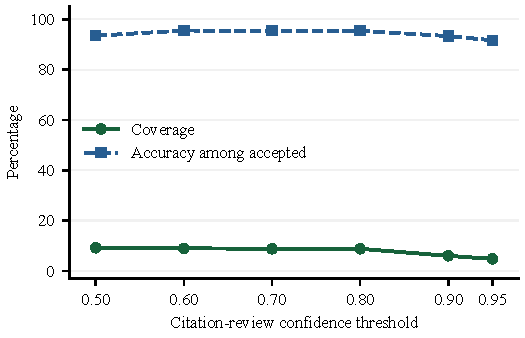
\includegraphics[width=\columnwidth]{acceptance-thresholds.pdf}
\caption{Semantic-threshold replay on 302 final assessments. The same evidence and structural rules are used throughout; this descriptive curve does not establish an optimal threshold.}
\label{fig:threshold}
\end{figure}

\subsection{Effect of Additional Research}
Across all workflow attempts, first-round accuracy is 69.5\pct, compared with 65.6\pct\ for final predictions. Forty predictions change: eight wrong-to-correct, twenty correct-to-wrong and twelve between incorrect labels. The final-minus-first difference is $-3.97$ percentage points (bootstrap 95\pct\ \CI: $-7.28$ to $-0.66$). Excluding five fatal attempts yields $-3.03$ points on 297 nonfatal attempts, with an interval of $-6.40$ to $0.00$.

Quota failures alone therefore do not explain the observed deterioration, although the nonfatal interval reaches zero. These trajectories do not establish that a separately deployed one-round system would behave identically: searches, timing and stopping can change under another protocol. Of the attempted workflows, 279 use three rounds, 15 use two and eight use one. The prevalence of the round limit warrants evaluating stopping behavior.

\subsection{Citation Diagnostics and Resource Use}
Final assessments contain 1,626 citation occurrences. Of these, 1,190 have literal quotes present in canonical text, and all 1,190 have Jev reviews. Fifteen reviewed quotes receive a relation other than \lq\lq supports,'' and 107 receive supporting confidence below 0.8. The remaining 436 occurrences fail literal provenance matching. They are not automatically counted as hallucinations: a quotation can refer to a snippet differing from the preferred full-page text, or exhibit another provenance mismatch.

Final structural gaps include missing exact quotations on 218 claims and insufficient independence flags on 224; these categories overlap. A host-exposure audit unwraps Wayback Machine URLs before comparison. On 134 of 302 claims, a cited host matches the host of the dataset's fact-check article. Host equality does not prove exact-article exposure, but published fact checks were available during retrieval.

\begin{table}[t]
\caption{Operational Measurements on Attempted Tasks}
\label{tab:cost}
\centering
\footnotesize
\begin{tabular}{@{}lrr@{}}
\toprule
Measurement & Full workflow & Model only\\
\midrule
Attempted tasks & 302 & 283\\
Fatal execution errors & 5 & 2\\
Mean elapsed time (s) & 81.2 & 5.6\\
Median elapsed time (s) & 78.4 & 3.6\\
90th percentile time (s) & 123.7 & 9.3\\
Logical search calls & 1,259 & 0\\
Page-fetch attempts & 2,460 & 0\\
Observed model tokens & 21,606,324 & 103,773\\
\bottomrule
\end{tabular}
\par\smallskip
\parbox{\columnwidth}{\scriptsize Different attempted samples: operational totals, not a paired cost estimate. Token accounting is incomplete; concurrent task durations are not study wall-clock time.}
\end{table}

Table~\ref{tab:cost} reports operational totals. There are 354 recorded fetch failures and two Jev ranking failures, distinct from seven fatal quota errors. The 573 rounds after the first consume 655 searches, 1,266 fetch attempts and 14,822,163 observed tokens; 153 add no new ledger records. Incomplete accounting prevents an exact monetary-cost estimate. Iteration cost and declining trace accuracy support investigating evidence novelty and stopping rules, rather than assuming more research is beneficial.

\section{Discussion and Limitations}
\subsection{What the Results Support}
The paired comparison offers preliminary evidence that the combined workflow improves label prediction over this control. Acceptance replay shows semantic checks removing wrong labels from a structurally eligible subset while also rejecting correct labels. Trace analysis identifies a cost-bearing failure mode in repeated research. These observations support treating prediction, acceptance and resource use as separate outcomes.

They do not establish a causal advantage of LangGraph over CrewAI, a hallucination-reduction percentage or benchmark-leading performance. No independently executed retrieval-only, Jev-disabled or alternative-framework condition has been completed. Fixed-assessment replay audits acceptance policy but cannot replace those experiments.

\subsection{Threats to Validity}
\textit{Interrupted execution:} The quota-limited subset can be affected by task order, latency and service availability. Its 177 matched claims cover only part of the split. Recorded errors are retained, and unexecuted tasks are not treated as successes or failures. The frozen conditions must be completed before finalizing benchmark-wide conclusions.

\textit{Temporal and verdict exposure:} Retrieval uses the contemporary web without a historical publication cutoff. Later reports and published verdicts can help predict older claims. Original AVeriTeC annotations address temporal evidence concerns \cite{averitec}, but our protocol does not reproduce that constraint. Pretraining exposure is unknown, and the repeatedly used development split is not a pristine held-out test.

\textit{Evidence validity:} Literal checks verify provenance only. Jev support judgments lack independent calibration and human entailment labels. Model-reported independence and peer-review flags can be wrong. Text similarity can miss paraphrased copying or flag legitimate overlap; snippets can omit qualifying context. The prepared human audit has not been performed.

\textit{Task and control scope:} Different prompts make the model-only comparison a combined-workflow effect. Heuristic decomposition can create incomplete fragments. Excluding \NEI\ from acceptance restricts task coverage. Multilingual, multimodal, adversarial and user-facing behavior has not been evaluated.

\textit{Reproducibility:} Hashes preserve source and text, not future service responses. Temperature zero does not guarantee bitwise reproducibility. Soft deadlines, incomplete token accounting and quotas affect measurements. Secrets are excluded from archived artifacts.

\subsection{Next Evaluation Steps}
The next computational step is to resume the remaining 415 tasks with the frozen model and configuration. Independent human review should assess citation support and source credibility. A separate study can compare one-round and iterative workflows under controlled retrieval and test stopping rules based on usable-evidence novelty rather than ledger growth. Such changes must be versioned and evaluated separately to avoid mixing post hoc improvements into this condition.

\section{Conclusion}
KajiAI makes proposed verdicts, evidence acceptance and research history independently inspectable. In an interrupted AVeriTeC development evaluation, the workflow improves paired label accuracy over a model-only control, while a strict gate accepts few claims and later research sometimes worsens predictions. The measured tradeoff concerns coverage, conditional correctness and cost. Completing the frozen study, validating citations independently and evaluating revised stopping policies remain necessary.

\section*{Acknowledgment}
OpenAI Codex assisted with drafting Sections I--VII, creating the architecture diagram and data-driven plotting code, and auditing evaluation scripts and regression tests. Numerical results were computed from saved execution records. Independent human citation validation was not performed. The authors are responsible for reviewing the manuscript, sources and findings before submission.

% Native IEEEtran last-page column balancing; no margin or body-font changes.
\IEEEtriggeratref{2}
\begin{thebibliography}{10}
\bibitem{fever}
J. Thorne, A. Vlachos, C. Christodoulopoulos, and A. Mittal, \lq\lq FEVER: A large-scale dataset for fact extraction and verification,'' in \emph{Proc. NAACL-HLT}, vol. 1, 2018, pp. 809--819, doi: 10.18653/v1/N18-1074.

\bibitem{averitec}
M. Schlichtkrull, Z. Guo, and A. Vlachos, \lq\lq AVeriTeC: A dataset for real-world claim verification with evidence from the web,'' in \emph{Advances in Neural Information Processing Systems}, vol. 36, 2023. [Online]. Available: \url{https://arxiv.org/abs/2305.13117}

\bibitem{sharedtask}
M. Schlichtkrull et al., \lq\lq The Automated Verification of Textual Claims (AVeriTeC) shared task,'' in \emph{Proc. Seventh Fact Extraction and VERification Workshop}, 2024, pp. 1--26, doi: 10.18653/v1/2024.fever-1.1.

\bibitem{rag}
P. Lewis et al., \lq\lq Retrieval-augmented generation for knowledge-intensive NLP tasks,'' in \emph{Advances in Neural Information Processing Systems}, vol. 33, 2020. [Online]. Available: \url{https://arxiv.org/abs/2005.11401}

\bibitem{alce}
T. Gao, H. Yen, J. Yu, and D. Chen, \lq\lq Enabling large language models to generate text with citations,'' in \emph{Proc. EMNLP}, 2023, pp. 6465--6488, doi: 10.18653/v1/2023.emnlp-main.398.

\bibitem{selfrag}
A. Asai, Z. Wu, Y. Wang, A. Sil, and H. Hajishirzi, \lq\lq Self-RAG: Learning to retrieve, generate, and critique through self-reflection,'' in \emph{Proc. International Conference on Learning Representations}, 2024. [Online]. Available: \url{https://arxiv.org/abs/2310.11511}

\bibitem{selective}
Y. Geifman and R. El-Yaniv, \lq\lq Selective classification for deep neural networks,'' in \emph{Advances in Neural Information Processing Systems}, vol. 30, 2017. [Online]. Available: \url{https://arxiv.org/abs/1705.08500}

\bibitem{langgraph}
LangChain, \lq\lq LangGraph overview.'' Accessed: Oct. 10, 2026. [Online]. Available: \url{https://docs.langchain.com/oss/python/langgraph/overview}
\end{thebibliography}
\end{document}

